\documentclass{beamer}
% % Example from http://www.math.umbc.edu/~rouben/beamer/quickstart-Z-H-3.html#node_sec_3
%\usepackage{default}
\usetheme{default}
\usepackage[utf8]{inputenc}  % this allows latex to understand UTF
                             % encoding in the file. This is
                             % important for Icelandic characters.
\usepackage[T1]{fontenc} % this enables icelandic characters in the output

% % Use the UMBC theme
% Template derived from hfc.tex by
% Rouben Rostamian <rostamian@umbc.edu>
% August 31, 2004 
\usetheme{ru1}
\useinnertheme{ruboxes}
\setbeamercolor{ruboxes}{bg=violet!12,fg=black}

\usepackage{rotating} % for defining \schwa
\newcommand{\schwa}{\raisebox{1ex}{\begin{turn}{180}e\end{turn}}}

\title{GeoLog}
\subtitle{Milestone presentation}
\author[P. Helgasson, S. Ólafsson, S. Magnússon, \& Þ. Tómasarson]{Páll Helgason pallsh12@ru.is, Sindri Ólafsson sindrio12@ru.is, Sveinn Elmar Magnússon sveinnm12@ru.is, \& Þór Tómasarson thortom12@ru.is}
\institute[RU]{
  Department of Science and Engineering (TVD) \\
  Reykjavík University \\
}
\date{October 28, 2014} %% Put the real presentation day so it doesn't
                        %% change later
\begin{document}

%----------- titlepage ----------------------------------------------%
\begin{frame}[plain]
  \titlepage
\end{frame}

%----------- slides ----------------------------------------------%
\begin{frame}{Presentation Hints}
Don't include these in your presentation, they are just here to help you.
\begin{itemize}
\item More pictures, less text.
\item Scan and look around the audience.
\item More slides, less time per slide.
\item Practice until you can do the slides without looking at them.
  If you must have notes, put them on cards.  Do not read from a page
  nor the slides.  It looks bad.
\item 45 -- 60 seconds per slide, no more.
\item Tell a story (make sure it flows).
\end{itemize}
\end{frame}

\begin{frame}{Introduction}
\begin{itemize}
% sett each as seperate slide...
\item Geological data collector
\item Collects data from multiple sensors and sends the data to the world wide web. 
\item Eases the observation of wide terrain
\item Andrew D. Wickert cares.
\end{itemize}
\end{frame}

\begin{frame}{Similar products}
\begin{itemize}
\item Automatic Weather Station (AANDERAA) \$ \cite{AANDERAA}
\item Computational Platform (BEAN) \$ \cite{BEAN}
\item Affordable Weather Stations \$1000 to \$2000 \cite{AffordableWS}
\end{itemize}
\centering
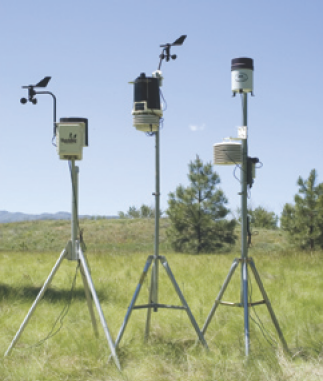
\includegraphics[height=3cm]{graphics/affordableWS.png}
\cite{AffordableWS}
\end{frame}

\begin{frame}{How is it better?}
\begin{itemize}
\item 
\end{itemize}
\end{frame}

\begin{frame}{Use case}
\begin{columns}[T] % contents are top vertically aligned
     \begin{column}[T]{7cm} % each column can also be its own environment
		\begin{itemize}
		\item Deployment of sensors
		\item Connect the sensors to communicators
			\begin{itemize}
			\item Wixel
			\item Xbee
			\item Any other wireless communicator
			\end{itemize}
		\item Position the main GeoLog module
		\item Connect to the Internet to see the incoming data
		\end{itemize}
	\end{column}
     \begin{column}[T]{3cm} % alternative top-align that's better for graphics
          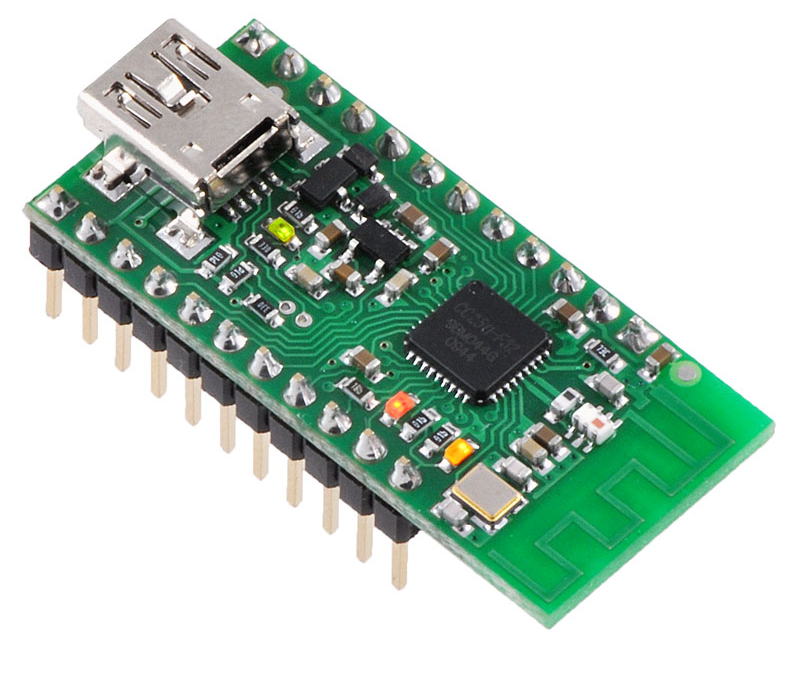
\includegraphics[height=3cm]{graphics/wixel.png}
          \cite{wixel}
     \end{column}
     \end{columns}
\end{frame}

\begin{frame}{Design: Overview}
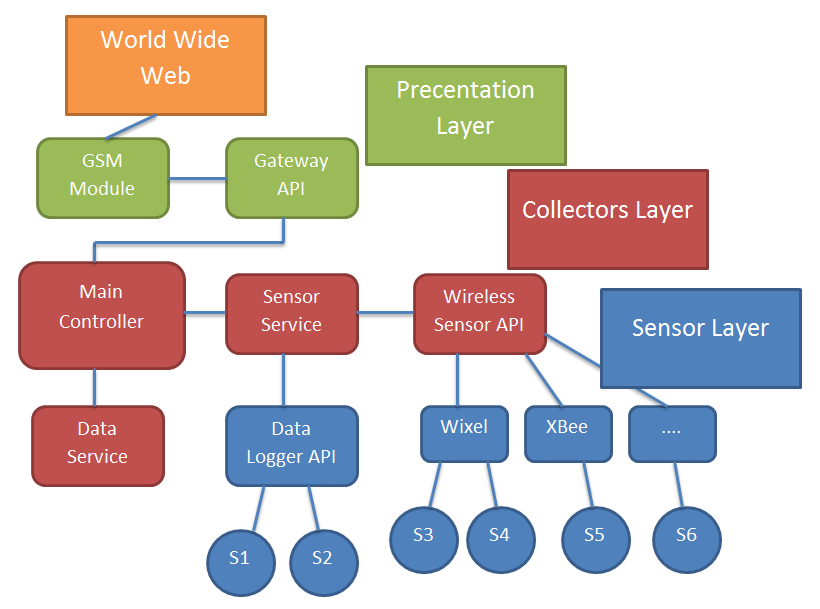
\includegraphics[height=8cm]{graphics/softwareArchitecture.png}
%What are the pieces of your design (software, hardware, etc.)  and how
%do they work together?  Put some pictures here to help explain what is
%going on.  Remember to cite all pictures and text using BibTeX.  If you cited
%the textbook\cite{carryer2011IntroMechatronics}, that is what it would
%look like.
\end{frame}

\begin{frame}{Design: Bill of materials (BOM)}
What are the electronics and materials?  What do they do? 

\begin{itemize}
\item 1 x Arduino Mega (Model: 2560 R3 from Sparkfun) \$45.95
\item 1 x GSM Module with shield  (Model: SM5100B from Sparkfun) \$99.95
\item 3 x Wixel   (With CC2511F32 microc. from Sparkfun) \$19.95
\item 3 x Sensors
\end{itemize}
\end{frame}

\begin{frame}{Status}
What have you done?  What is the current state?  Is there any interesting/hard problems
that need to be solved?  How are you going to solve them?
\end{frame}

\begin{frame}{Tasks remaining}
What is left to be done?  This should be broken down by the time remaining in class.
\end{frame}

\begin{frame}{References}
Thank you for your time.
Questions?
\bibliographystyle{IEEEtran}
\bibliography{references}
\end{frame}

\end{document}
